\documentclass[11pt]{article} 
\usepackage[utf8]{inputenc}

%%% PAGE DIMENSIONS
\usepackage{geometry}
\geometry{a4paper}

\usepackage{graphicx} % support the \includegraphics command and options

% \usepackage[parfill]{parskip} % Activate to begin paragraphs with an empty line rather than an indent

%%% PACKAGES
\usepackage{float}
\usepackage{booktabs}
\usepackage{array}
\usepackage{paralist}
\usepackage{verbatim}
\usepackage{subfig} 
\usepackage{fancyhdr}


\pagestyle{fancy} % options: empty , plain , fancy
\renewcommand{\headrulewidth}{0pt} % customise the layout...
\lhead{}\chead{}\rhead{}
\lfoot{}\cfoot{\thepage}\rfoot{}

\usepackage{sectsty}
\allsectionsfont{\sffamily\mdseries\upshape}

\usepackage{listings}
\usepackage{color}

\definecolor{mygreen}{rgb}{0,0.6,0}
\definecolor{mygray}{rgb}{0.5,0.5,0.5}
\definecolor{mymauve}{rgb}{0.58,0,0.82}

\lstset{ 
  backgroundcolor=\color{white},   % choose the background color; you must add \usepackage{color} or \usepackage{xcolor}; should come as last argument
  basicstyle=\footnotesize,        % the size of the fonts that are used for the code
  breakatwhitespace=false,         % sets if automatic breaks should only happen at whitespace
  breaklines=true,                 % sets automatic line breaking
  captionpos=b,                    % sets the caption-position to bottom
  commentstyle=\color{mygreen},    % comment style
  firstnumber=1000,                % start line enumeration with line 1000
  frame=single,	                   % adds a frame around the code
  keepspaces=true,                 % keeps spaces in text, useful for keeping indentation of code (possibly needs columns=flexible)
  keywordstyle=\color{blue},       % keyword style
  language=Python,                 % the language of the code
  numbers=left,                    % where to put the line-numbers; possible values are (none, left, right)
  numbersep=5pt,                   % how far the line-numbers are from the code
  numberstyle=\tiny\color{mygray}, % the style that is used for the line-numbers
  rulecolor=\color{black},         % if not set, the frame-color may be changed on line-breaks within not-black text (e.g. comments (green here))
  showspaces=false,                % show spaces everywhere adding particular underscores; it overrides 'showstringspaces'
  showstringspaces=false,          % underline spaces within strings only
  showtabs=true,                   % show tabs within strings adding particular underscores
  stepnumber=1,                    % the step between two line-numbers. If it's 1, each line will be numbered
  stringstyle=\color{mymauve},     % string literal style
  tabsize=2,	                   % sets default tabsize to 2 spaces
  title=\lstname                   % show the filename of files included with \lstinputlisting; also try caption instead of title
}


\title{Práctica 0: Python}
\author{Ana Martín Sánchez, Nicolás Pastore Burgos}
\date{21/09/2021} 

\begin{document}
\maketitle

\section{Descripción de la práctica}

 En esta práctica, se pedía un algoritmo de integración numérica, basado en el método de Monte Carlo. Este método de consiste en calcular probabilidades utilizando secuencias de números aleatorios. 

 Es decir, en lugar de calcular la integral de una función entre dos puntos, se busca el valor máximo M en el intervalo [f(a), f(b)], y generamos un rectángulo de anchura (b-a) y altura M. A partir de este punto, entra en juego el método de Monte Carlo; generamos puntos aleatorios dentro de ese rectángulo, y observamos si caen por debajo de la función. Repitiendo este proceso, podemos hacer una aproximación del valor de la integral.

 Al utilizar el algoritmo que se pide implementar, un posible resultado sería el de la figura 1.
 
 \begin{figure}[h!]
    \begin{center}
    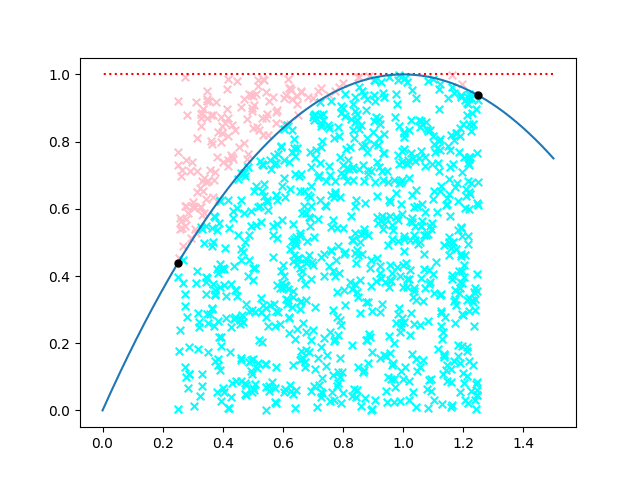
\includegraphics[width=0.4\textwidth]{EjemploMonteCarlo.png}
    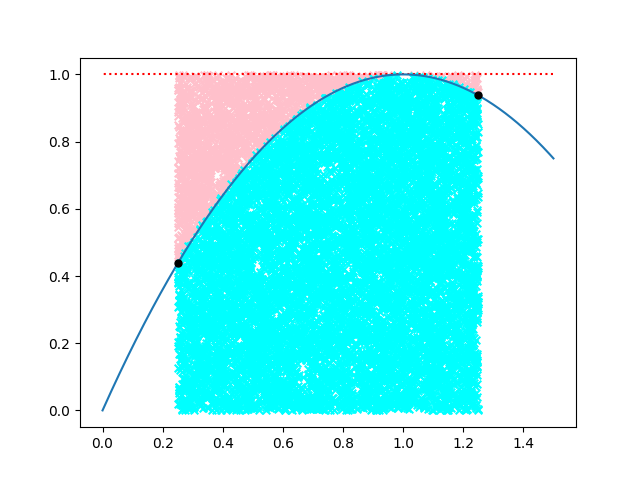
\includegraphics[width=0.4\textwidth]{EjemploMonteCarlo2.png}
    \caption{Después de buscar puntos aleatorios, y comprobar cuáles están por debajo de la función, podemos intuir cuál es la integral de dicha función. Cuantos más puntos calculemos, más cercana a la realidad es la aproximación que se hace.}
    \label{fig:EjemploMonteCarlo}
    \end{center}
 \end{figure}

 Además, para la práctica se pide hacer dos versiones del mismo algoritmo: una iterativa, con bucles; y otra que opere sobre vecotres, con el fin de calcular los tiempos de ejecución obtenidos con ambas versiones. Es importante recordar que esta diferencia se hará más notable cuanto mayor sea el número de puntos generados.
\newpage
\section{Solución propuesta}

\subsection{Resultados obtenidos}

 Tras varias pruebas, se puede observar que el tiempo consumido al utilizar vectores está en el orden O(1). Es decir, se mantiene prácticamente constante, independientemente del número de puntos calculados para obtener la integral.

 Sin embargo, al utilizar bucles for, el tiempo está en el orden O(n). Cuantos más puntos se crean, mayor es el recorrido del bucle; por tanto, se tarda más tiempo en recorrer todos los puntos.

 En la figura 2 se ve un ejemplo de ejecución, en el que se ven los tiempos necesarios para obtener la integral. En el eje X de la gráfica, se indican el número de puntos creados; en el eje Y, el tiempo consumido por cada algoritmo, en nanosegundos. Además, como se lee en la leyenda, en azul se muestran los resultados obtenidos con el algoritmo basado en bucles y, en rojo, los obtenidos con el algoritmo basado en vectores.
 
 \begin{figure}[h!]
    \begin{center}
    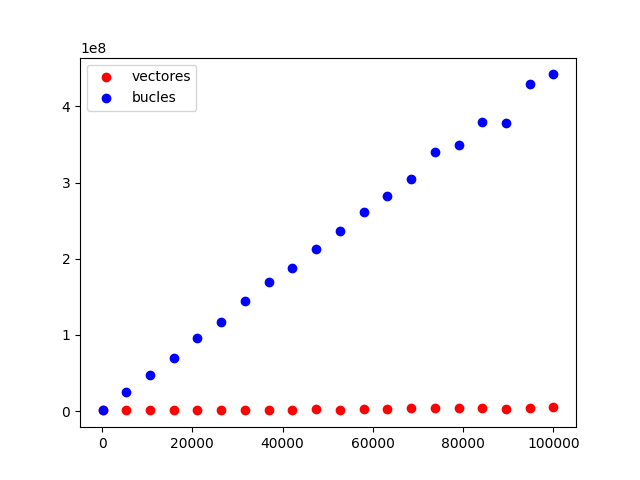
\includegraphics[width=\textwidth]{Resultados.png}
    \caption{Se puede observar cómo, a medida que el número de puntos calculados aumenta, la diferencia de tiempos se hace mayor.}
    \label{fig:Resultados}
    \end{center}
 \end{figure}
\subsection{Implementación}

\lstinputlisting[language=Python]{main.py}


\end{document}
